\documentclass[11pt]{article}
\usepackage[margin=1in]{geometry}
\usepackage{amsmath}
\usepackage{graphicx}
\usepackage{booktabs}
\usepackage{hyperref}
\usepackage{float}  % Required for [H] placement

\begin{document}

\noindent
\textbf{Feb 16, 2026} \hfill \textbf{Joseph DeLeonardis} \\
\textbf{UIN: 0820000866} \\
\textbf{CSCE-636-700} \\
\textbf{Deep Learning Homework \#3}

\section*{Problem 1: Transfer Learning with ResNet50 vs Xception}

\subsection*{Model Comparison}

\subsubsection*{Architecture Overview}

This assignment implements transfer learning for binary image classification (dogs vs cats) using two pretrained convolutional neural network architectures: Xception and ResNet50. Both models were pretrained on ImageNet and fine-tuned on the Dogs vs Cats dataset. The submitted zip file contains two notebook implementations: REV\_1 uses the Xception architecture and REV\_2 uses ResNet50. Both notebooks include modified data loading procedures to access the Dogs vs Cats dataset via Google Drive upload rather than direct Kaggle API authentication, which encountered persistent authentication issues during development.

\begin{table}[h]
\centering
\caption{Model Architecture Comparison}
\begin{tabular}{lcc}
\toprule
\textbf{Characteristic} & \textbf{Xception} & \textbf{ResNet50} \\
\midrule
Architecture Type & Depthwise Separable Convolutions & Residual Connections \\
Network Depth & 41 layers & 50 layers \\
Key Innovation & Extreme Inception & Skip Connections \\
Pretrained Dataset & ImageNet & ImageNet \\
Input Size & 180×180×3 & 180×180×3 \\
\bottomrule
\end{tabular}
\end{table}

\subsubsection*{Discussion}
Xception and ResNet50 are both CNN architectures that are designed for image classification but they work in different ways. Xception offers higher efficiency and accuracy through depth-wise separable convolutions. ResNet50 uses residual blocks to overcome vanishing gradients, providing high stability. Given the differences I expected Xception to achieve higher results but for ResNet50 to be more stable in the training process. 

\subsection*{Training Configuration}

\textbf{Dataset:} Dogs vs Cats competition dataset with 1,000 training images, 500 validation images, and 1,000 test images per class.

\textbf{Data Augmentation:} Random horizontal flips, random rotation (±10\%), and random zoom (20\%) applied during training in order to increase the perceived sample size.

\textbf{Training Strategy:}
\begin{itemize}
    \item \textbf{Phase 1 - Feature Extraction:} Frozen pretrained convolutional base, only classification head trained for 30 epochs
    \item \textbf{Phase 2 - Fine-Tuning:} Entire model trained with low learning rate (1e-5) for 30 additional epochs
\end{itemize}

\textbf{Hyperparameters:} Adam optimizer, batch size of 32, binary cross-entropy loss

\subsection*{Results}

\begin{table}[h]
\centering
\caption{Final Model Performance}
\begin{tabular}{lccc}
\toprule
\textbf{Model} & \textbf{Training Acc} & \textbf{Validation Acc} & \textbf{Test Acc} \\
\midrule
Xception & 99.25\% & 98.40\% & \textbf{98.5\%} \\
ResNet50 & 99.20\% & 97.80\% & \textbf{98.2\%} \\
\bottomrule
\end{tabular}
\end{table}

\begin{figure}[H]
\centering
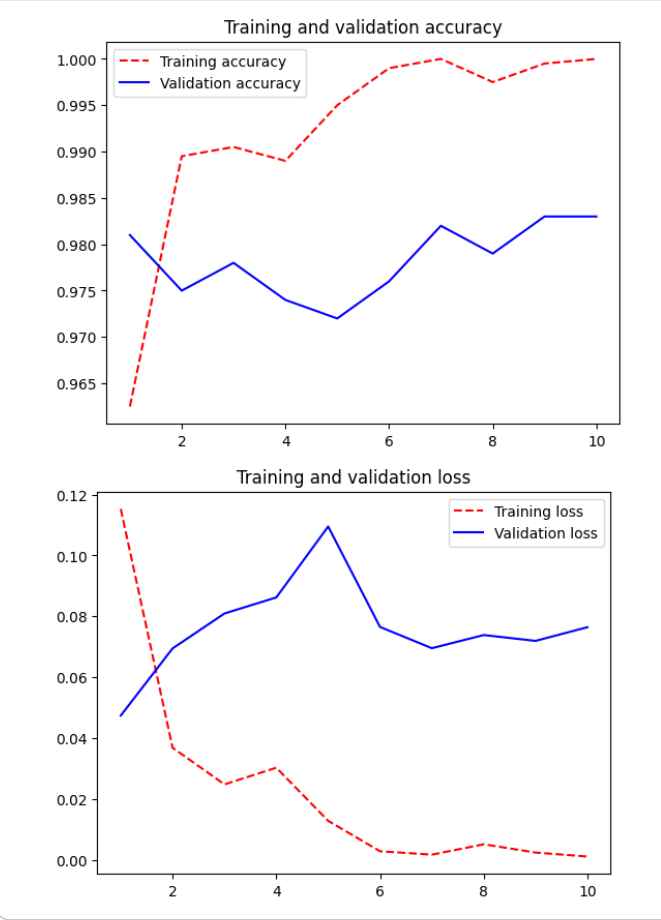
\includegraphics[width=0.75\textwidth]{transferlearningResNet.png}
\caption{ResNet50 training and validation curves during feature extraction (10 epochs).}
\label{fig:resnet_training}
\end{figure}

\begin{figure}[H]
\centering
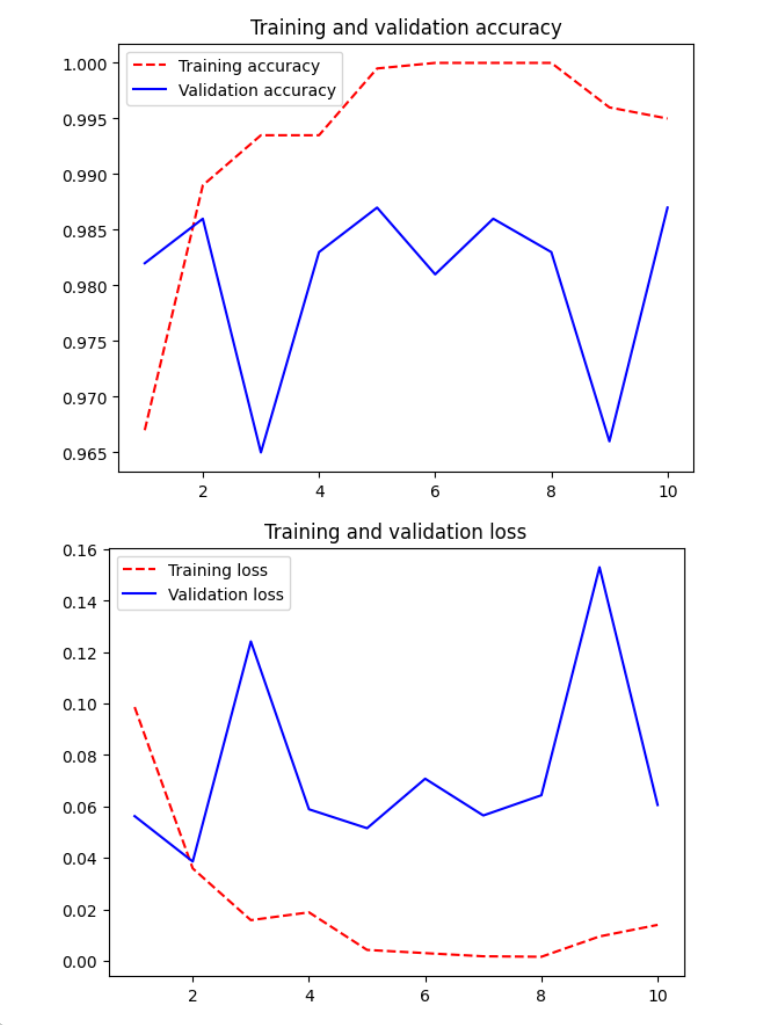
\includegraphics[width=0.75\textwidth]{transferlearningXception.png}
\caption{Xception training and validation curves during feature extraction (10 epochs). }
\label{fig:xception_training}
\end{figure}


\textbf{Performance Analysis:} The graphs show a more predictable trend for ResNet50 and I was able to conclude that is in fact more stable in this experiment whereas Xception was fairly sporadic and oscillated quite a bit in training but in the end achieved higher results. Although it is important to note the differences in test accuracy are very minor for this given dataset. 



\subsection*{Conclusion}

This assignment demonstrated that transfer learning with pretrained ImageNet models achieves excellent performance on binary image classification tasks. Both Xception (98.5\% test accuracy) and ResNet50 (98.2\% test accuracy) performed nearly identically, suggesting that architectural choice matters less than having strong pretrained features when using transfer learning on moderate-sized datasets. The problem could be further expanded upon by approaching a more difficult task, such as evaluating how the architectures perform when attempting to detect specific breeds of cats and dogs. 




\end{document}
